% Chapter 4

\chapter{Models Capture the Smile} % Main chapter title

\label{Chapter4} % For referencing the chapter elsewhere, use \ref{Chapter1} 
% Define some commands to keep the formatting separated from the content 
%\newcommand{\keyword}[4]{\textbf{#4}}
%\newcommand{\tabhead}[4]{\textbf{#4}}
%\newcommand{\code}[4]{\texttt{#2}}
%\newcommand{\file}[4]{\texttt{\bfseries#4}}
%\newcommand{\option}[4]{\texttt{\itshape#4}}

%----------------------------------------------------------------------------------------
Enormous body of research have been conducted on the volatility models, largely motivated by its importance in financial market. The volatility of a financial instrument is often seen as one of the most important risk indicators as well as a key parameter in many pricing models in financial market. In this section we first review local volatility (LV) models and stochastic volatility (SV) models. In the class of  local volatility models, we start with the Dupire's local volatility model which is a generalisation of the classic Black-Scholes model \parencite{bs1973} and then move to Displaced Diffusion model introduced by Rubinstein \parencite{displaced_process} which generates a sloping implied skew to the original model. Then we proceed to a class of stochastic volatility models where volatility is driven by an additional stochastic differential equation. The most popular ones among financial institutions include Heston model \parencite{Heston1993ACS} in which the randomness of the variance process varies as the square root of variance, Constant Elasticity of Variance (CEV) discussed by Cox and Ross \parencite{cox1975notes} which attempts to capture both stochastic volatility and the leverage effect.   Despite this two classes of models have the capability of capturing the smile features, they are insufficient to describe the asymptotic behaviour of the entire smile surface. This leads to the development of the stochastic local volatility (SLV) models. This class of hybrid model includes both stochastic and local volatility as its name suggests. In this model, the volatility from the stochastic volatility model can be modified with a local volatility function. Under such a construction, SLV models allow quick calibration to plain-vanilla options with the potential to extend to exotic options. 



%----------------------------------------------------------------------------------------
\section{Black-Scholes Model}
A major breakthrough in the option pricing world is made by Fisher Black and Myron Scholes \parencite{bs1973} in 1973. They developed a model for pricing a financial derivative. This model 
estimates the evolution of a price of an underlying overtime. It assumes the price of the underlying asset follows a Geometric Brownian motion under the risk-neutral measure, defined as :
\begin{equation}
\label{eqn:GBM}
dS_{t}=r S_{t}\,dt+\sigma S_{t}\,dW_{t}
\end{equation}
Where
$W_{t}$ is a Wiener process or Brownian motion,  $r$ is the risk-free rate served as 'the percentage drift' and constant volatility $\sigma$.\\

In particular, they derived a differential equation given in Equation~\ref{eqn:bls_pde} governing the price $ V(S, t)$evolution of the option under the model by applying \textit{It\^{o}}'s lemma for two variables in Equation~\ref{eqn:GBM} . 
 \begin{equation}
 \label{eqn:bls_pde}
dV=\left(\mu S{\frac {\partial V}{\partial S}}+{\frac {\partial V}{\partial t}}+{\frac {1}{2}}\sigma ^{2}S^{2}{\frac {\partial ^{2}V}{\partial S^{2}}}\right)dt+\sigma S{\frac {\partial V}{\partial S}}\,dW
\end{equation}

By solving the PDE for the corresponding terminal and boundary conditions as stated below:
\begin{align}
C(S, T) = max(S-K, 0)\\
C(0, t) = 0\\
C(\infty,t) \approx S
\end{align}
 Where $T$ is the maturity, and $K$ is the strike.
 
We have an analytic solution for European call option price given by:

 \begin{equation}
 \label{eqn:bls}
C(S_{t},t) =N(d_{1})S_{t}-N(d_{2})Ke^{-r(T-t)},
\end{equation}
with
\begin{align}
d_{1}&={\frac {1}{\sigma {\sqrt {T-t}}}}\left[\ln \left({\frac {S_{t}}{K}}\right)+\left(r+{\frac {\sigma ^{2}}{2}}\right)(T-t)\right]\\
d_{2}&=d_{1}-\sigma {\sqrt {T-t}}.
 \end{align}
where $N(x)$ denotes the standard normal cumulative distribution function

\begin{equation}
 N(x)={\frac {1}{\sqrt {2\pi }}}\int _{-\infty }^{x}e^{-z^{2}/2}\,dz.
\end{equation}
Specifically, $N(d_2)$ is the probability that the call will be exercised under the assumption that the underlying asset has the risk-free rate.

 Black-Scholes Model provides the possibility to price European options in a quick and elegant manner. 
 However, in reality, the price of underlying asset does not always follow a GBM, there are occasionally jumps in the movement of the price. Asset prices also tend to have heavier tails than log-normal distribution as predicted in GBM. This discrepancy leads to the Black-Scholes model substantially underpricing or overpricing an option. For more complicated options than plain vanilla option or more general assumptions, we require numerical methods for pricing. For example, if the underlying asset pays dividends or the interest rate is not constant, we may employ finite difference methods or tree approach. For the valuation of options with multiple sources of uncertainty or with complicated features, Monte Carlo methods are employed. Further developments of the model revolve around mainly two directions. The first one engages into extending Black-Scholes framework by incorporating stochastic jumps or stochastic volatility, famous work includes jump-diffusion and general Levy process models, see paper by Merton \parencite{merton1976}, Kou \parencite{kou2002} and Bates\parencite{bates1996};   the second one estimates the stochastic density function of the underlying asset directly from the market option prices, for example, Dupire's model \parencite{Dupire}.
%-----------------------------------------------------------------------------------------
 \subsection{Implied Volatility }
 The implied volatility can be interpreted as the volatility implied by the market quoted plain vanilla option prices under a certain model assumption. In other words, the implied volatility is implicitly contained in the market quote\parencite{alexander1996}. 
 
 In the Black-Scholes framework, the implied volatility $\sigma_\text{imp}(K, T)$ is given by equaling the Black Scholes formula~\ref{eqn:bls} to the current market call price.  \begin{equation}
 C_\text{mkt}(S,K,T) = C_\text{bls}(S,K,T,r,\sigma(K, T)))
 \end{equation}
 
 where $C_\text{mkt}(S,K,T)$ denotes the current market price of a call option with maturity $T$ and strike $K$, and $C_\text{bls}$ is the price given by the Black-Scholes formula. There is no closed form analytical solution for this equation, however, numerical approaches like, Newton-Raphson Method , Bisection Method where the latter one does not require the computation of Vega (derivative of call price w.r.t $sigma$) and is extendable to American style options.  Although, Newton-Raphson Method does not provide accurate approximation for options with very Away-From-Money strikes, it remains the dominating method in this area. 
 
Since the Black-Scholes formula is monotonically increasing in $\sigma$, there will always be a unique solution, $\sigma(K,T)$ for the given market price $C_\text{mkt}$ under the arbitrage free assumption. This implies, in the Black-Scholes framework, the volatility is constant for all strikes $K$ and maturity $T$ which means a flat volatility surface. However, this is hardly the case in practice. In fact, the market has long observed the dependence between volatility and both strikes and maturities. 
 The plot of volatilities against strikes are commonly known as 'volatility smile', 'volatility smirk' or 'volatility frown' depends on the shape. A volatility smile suggests higher implied volatilities for deep in-the-money and out-of-money options. This is only observed after the market crush of 1978\parencite{hull2006} and  is believed to be resulted from that investor reassessments of the probabilities of fat-tail have led to higher prices for out-of-the-money options. In order to account for this high price we need a relatively high implied volatilise. In equity market, the resulting plot is typically downward sloping or a small tilted smile with a kink observed near the money, in such cases the graphs are described as 'a volatility skew' or 'a volatility smirk'.

To accurately describe the market reality, in particular the 'volatility skew', a wide range of models have been developed in the past decades. This brings us to the discussion of local volatility models and stochastic volatility models in the following sections.

 
%------------------------------------------------------------------------------------------
\section{Local volatility Model}
A local volatility model, in mathematical finance and financial engineering context, calculates the volatilities as a function of underlying spot price $S(t)$ and of time $t$. It is a generalisation of the classic Black-Scholes model, in which the volatility is assumed to be constant rather than time-varying.
Under standard assumption of arbitrage-free market, the resultant option prices from the local-volatility model should match market prices. The two key developments in this field are "Implied binomial trees" by Emanuel Derman and Iraj Kani \parencite{BinoTree} and the Dupire's formula by Bruno Dupire \parencite{Dupire}.  These approaches allow the calibration of the volatility surface from implied volatilities and a one factor Black-Scholes model. In such a manner, local volatility values for all combinations of strike prices and expiration dates are attainable from the generated volatility surface.
The main advantage of the LV models is that they provide an exact and fast calibration to the volatility surface of European options through an analytical formula. However, when local volatility was first introduced, the authors did not see them as a separate class of models that represented the evolution of the volatilities. Rather, it can be proved that local variance is indeed a risk-neutral expectation of instantaneous variance\footnote{Detailed proof steps can be found in Gatheral, Jim. (2003). Lecture 1: Stochastic Volatility and Local Volatility in section 2.5. }. 
%----------------------------------------------------------------------------------------

\subsection{Implied Tree Model}
Derman and Kani\parencite{Derman1994}proposed an implied tree model to account for the 'volatility smile' phenomenon as we mentioned in the previous section. In their model construction, the future underlying asset prices are estimated by a random walk use the strikes and expirations of the options as input. They showed in their paper, how a unique binomial tree is extracted from the 'volatility smile' and hence be used to value any kind of options consistently with the market. The tree model also produces the distribution and the volatilities of the underlying asset implied by the option prices at market levels. 
In the implied binomial tree model, $n$ levels are uniformed spaced, with $\delta t$ apart and a time-varying risk-free interest rate $r$( level index is avoid for notational simplicity) at each level. At $i^{th}$ node in level $n$, the asset price is known as $s_i$ and evolves to an up node $S_{i+1}$ with probability $p_i$ and to a down node$S_i$ with probability $1-p_i$ at $n+1$ level. The corresponding Arrow-Debreu price \footnote{ Risk-neutral expectation of the discounted payoff.}to $s_i$ is $\lambda_i$ and forward price is $e^{r\delta t}s_i$. The illustration of the structure of the tree can be found in Figure~\ref{fig:tree}.
\begin{figure}
\centering
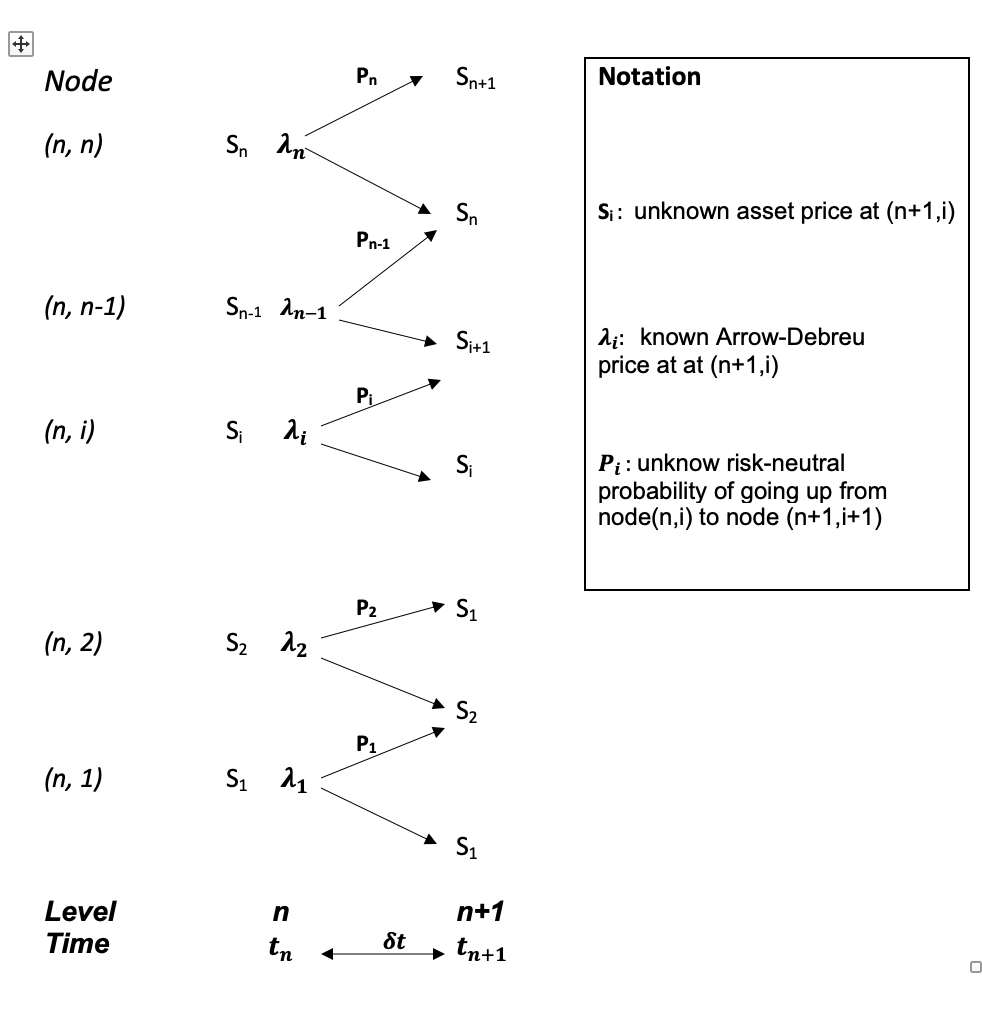
\includegraphics[width=0.5\columnwidth]{Figures/tree}
\decoRule
\caption{Constructing the $(n+1)^{th}$ Level of the Implied Tree}
\label{fig:tree}
\end{figure}
Under the risk-neutral assumption in the Binomial tree structure, the expected asset price one period ahead must agree with the forward price $F-i$:
\begin{equation}
\label{eqn:foward}
F_i = p_i S_{i+1} +(1-p_i)S_{i}
\end{equation}

Let $C(s_i, t_{n+1})$ and $P(s_i, t_{n+1})$ denote the market call and put prices struck today at $s_i$ and expiring at $t_{n+1}$ then those prices can be obtained by interpolating the smile structure at time $t_{n+1}$. Call option price with strike K, can be calculated by summing up the discounted payoff multiplied by the corresponding probabilities of reaching each note in the next step:
\begin{equation}
\label{eqn:call_tree}
C(K, t_{n+1}) = e^{-r \delta t} \sum_{j=1}^n {\lambda_j p_j +\lambda_{j+1}(1- p_{j+1})} \text{max} (S_{j+1}-K, 0)
\end{equation}
when the option is at the money, e.g $K= s_i$, Equation ~\ref{eqn:call_tree}, using the forward price equation, can be rewritten as:

\begin{equation}
\label{eqn:re_tree}
e^{r \delta t}C(s_i, t_{n+1}) =   \lambda_i p_i (S_{i+1}-s_i)+\sum_{j=1}^n \lambda_{j}(F_j- s_i)
\end{equation}

Since both $C(s_i, t_{n+1})$ and $F_i$ are known, $S_{i+1}$ and $p_i$ can be solved with Equation 
~\ref{eqn:foward} and Equation~\ref{eqn:re_tree}.

\begin{align}
\label{eqn:iterative}
S_{i+1} = \frac{S_i[e^{r\delta t}C(s_i, t_{n+1})-\sum_{j=1}^n \lambda_{j}(F_j- s_i)]-\lambda_i s_i(F_i-S_i) }{[e^{r\delta t} C(s_i, t_{n+1})-\sum_{j=1}^n \lambda_{j}(F_j- s_i)]-\lambda_i (F_i-S_i)}\\
p_i = \frac{F_i -S_i}{S_{i+1}-S_i}
\end{align}

Iteratively, in this manner, we can find the prices and 'up' and 'down' probabilities in each node above the centre of the tree given the known initial node.

In particular, if the number of the nodes in $n+1^{th}$ node is odd, then we set initial $S_i$ with $i=n/2 +1$ with the spot price $s_i$at the central node. Use equations in ~\ref{eqn:iterative} we can cover each node in upper half of the tree.  

if the number of the nodes in $n+1^{th}$ node is even, we start with the nodes just above and below the central level, $S_{i+1}$ and $S_i$ respectively. This two nodes need to satisfy the condition $S_i = \frac{s_i^2}{S_{i+1}}$. Together with Equation~\ref{eqn:call_tree} we have:
\begin{equation}
S_{i+1} = \frac{s_i[e^{r\delta} t C(s_i, t_{n+1})+\lambda_i s_i -\sum_{j=1}^n \lambda_{j}(F_j- s_i)]}{\lambda_i F_i - e^{r\delta t} C(s_i, t_{n+1})+\sum_{j=1}^n \lambda_{j}(F_j- s_i)} \quad\quad\quad for \quad i =n/2
\end{equation}
Similarly, we construct the lower part of the tree iteratively use:
\begin{equation}
S_{i} = \frac{S_{i+1}[e^{r\delta} t P(s_i, t_{n+1})-\sum_{j=1}^n \lambda_{j}(F_j- s_i)]+\lambda_i s_i(F_i-S_{i+1})}{[e^{r\delta t} P(s_i, t_{n+1})-\sum_{j=1}^n \lambda_{j}(F_j- s_i)]+\lambda_i (F_i-S_{i+1})} 
\end{equation}
Hence, the implied local volatility $\sigma(S,t)$ is reflected in the implied binomial tree.




%----------------------------------------------------------------------------------------


%----------------------------------------------------------------------------------------

%----------------------------------------------------------------------------------------


